\subsection{Adjusted Mutual Information evolution over number of zernike modes}

	\subsubsection{AMI evolution over number of clusters for 2 zernike mode related datasets}
		\begin{figure*}[ht!]
			\centering
			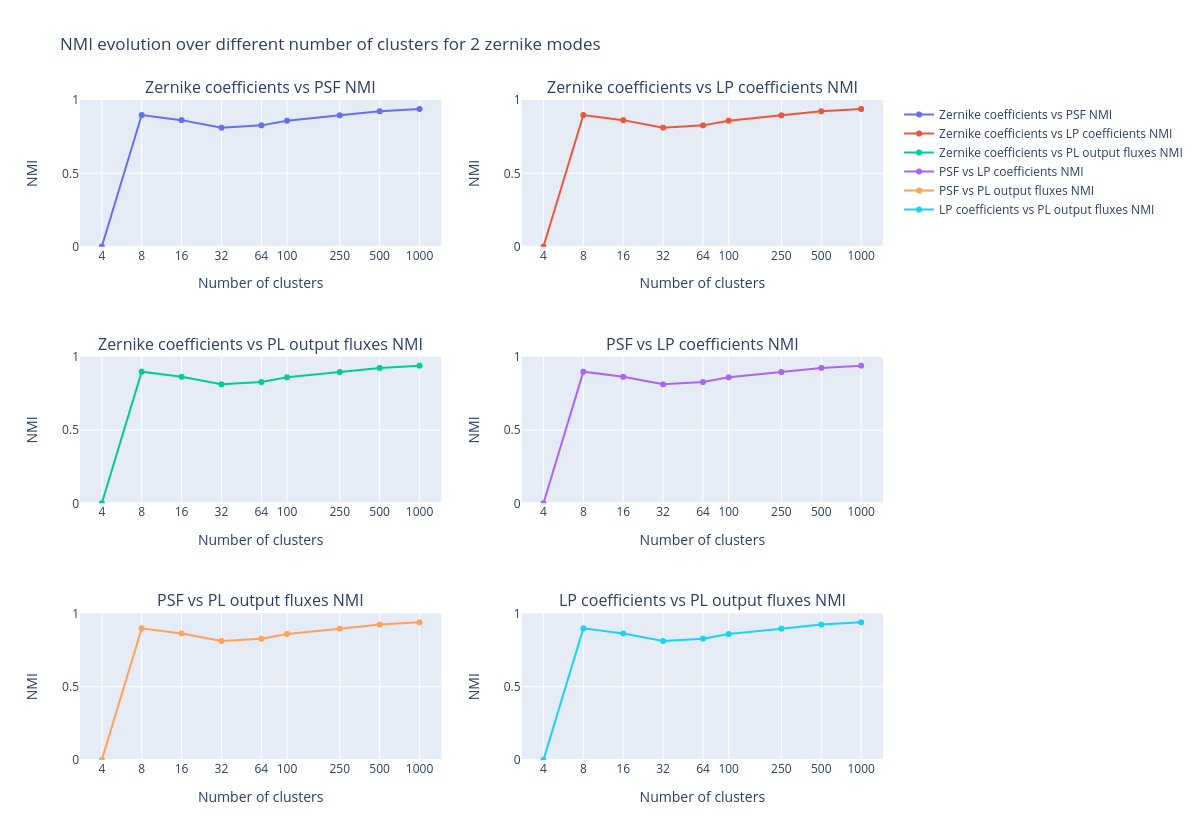
\includegraphics[width=0.9\textwidth]{nmia-nmievolutionover2.png}
		\end{figure*}
		\begin{table}[!h]
		\centering
		\begin{tabular}{|c|c|c|c|c|c|c|}
\hline
\textbf{Clusters} & \textbf{Z vs PSF} & \textbf{Z vs LP} & \textbf{Z vs PL} & \textbf{PSF vs LP} & \textbf{PSF vs PL} & \textbf{LP vs PL} \\
\hline
4   & 0.9248 & 0.9342 & 0.6276 & 0.8917 & 0.6037 & 0.6370 \\
8   & 0.9206 & 0.9101 & 0.6317 & 0.8921 & 0.6291 & 0.6483 \\
16  & 0.8713 & 0.8956 & 0.7641 & 0.8558 & 0.7538 & 0.8006 \\
32  & 0.7866 & 0.8873 & 0.7635 & 0.7670 & 0.7519 & 0.7594 \\
64  & 0.8245 & 0.8421 & 0.8130 & 0.8290 & 0.7954 & 0.8312 \\
100 & 0.8289 & 0.8414 & 0.8051 & 0.8254 & 0.8043 & 0.8240 \\
250 & 0.8064 & 0.7804 & 0.7630 & 0.8115 & 0.7843 & 0.7874 \\
500 & 0.7871 & 0.7813 & 0.7506 & 0.7858 & 0.7595 & 0.7712 \\
1000& 0.7473 & 0.7666 & 0.7436 & 0.7287 & 0.7162 & 0.7639 \\
2000& 0.7022 & 0.7929 & 0.7454 & 0.6813 & 0.6569 & 0.7705 \\
\hline
\end{tabular}
\caption{AMI Analysis for Different Numbers of Clusters}
\end{table}		
		\FloatBarrier
		
	\subsubsection{AMI evolution over number of clusters for 5 zernike mode related datasets}
		\begin{figure*}[ht!]
			\centering
			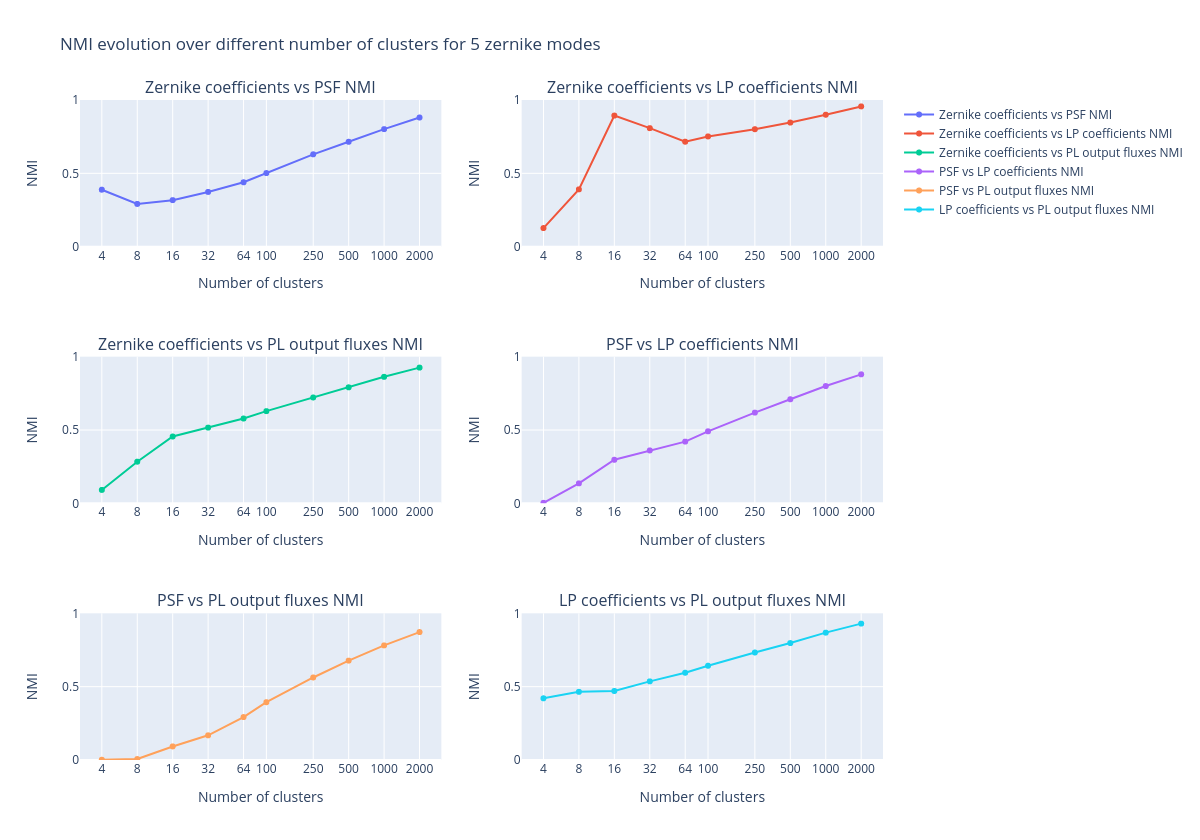
\includegraphics[width=0.9\textwidth]{nmia-nmievolutionover5.png}
		\end{figure*}
		
		\begin{table}[h!]
\centering
\begin{tabular}{|c|c|c|c|c|c|c|}
\hline
\textbf{Clusters} & \textbf{Z vs PSF} & \textbf{Z vs LP} & \textbf{Z vs PL} & \textbf{PSF vs LP} & \textbf{PSF vs PL} & \textbf{LP vs PL} \\
\hline
4   & 0.3880 & 0.1263 & 0.0908 & 0.0027 & 0.0010 & 0.4204 \\ \hline
8   & 0.2896 & 0.3890 & 0.2821 & 0.1341 & 0.0040 & 0.4636 \\ \hline
16  & 0.3116 & 0.8930 & 0.4510 & 0.2912 & 0.0849 & 0.4661 \\ \hline
32  & 0.3542 & 0.8022 & 0.5016 & 0.3412 & 0.1430 & 0.5221 \\ \hline
64  & 0.3694 & 0.6800 & 0.5256 & 0.3489 & 0.2051 & 0.5445 \\ \hline
100 & 0.3675 & 0.6836 & 0.5279 & 0.3542 & 0.2321 & 0.5459 \\ \hline
250 & 0.3178 & 0.6305 & 0.4855 & 0.2979 & 0.1973 & 0.5063 \\ \hline
500 & 0.2525 & 0.5929 & 0.4476 & 0.2379 & 0.1551 & 0.4641 \\ \hline
1000 & 0.2000 & 0.5881 & 0.4392 & 0.1933 & 0.1241 & 0.4625 \\ \hline
2000 & 0.1549 & 0.6806 & 0.4585 & 0.1452 & 0.0972 & 0.4893 \\ \hline

\hline
\end{tabular}
\caption{AMI Analysis for Different Numbers of Clusters}
\end{table}
		\FloatBarrier
		
	\subsubsection{AMI evolution over number of clusters for 9 zernike mode related datasets}
		\begin{figure*}[ht!]
			\centering
			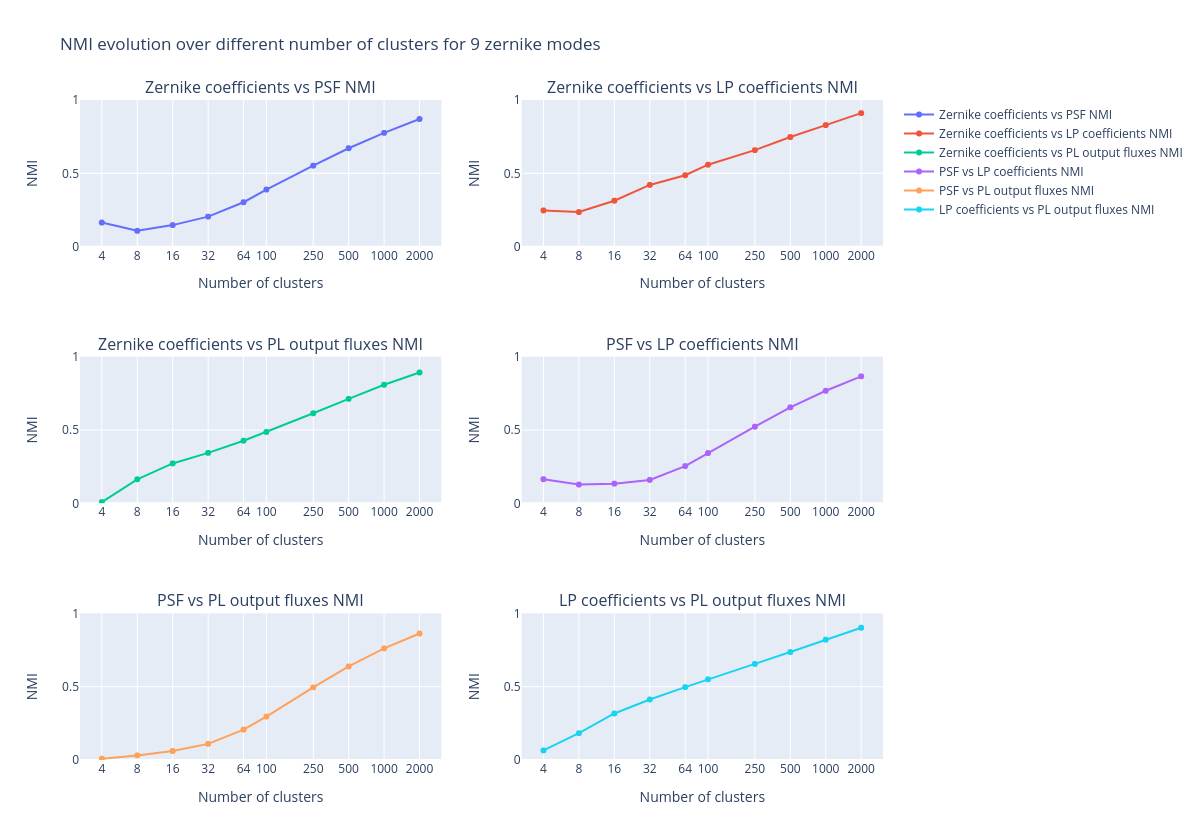
\includegraphics[width=0.9\textwidth]{nmia-nmievolutionover9.png}
		\end{figure*}

\begin{table}[h!]
\centering
\begin{tabular}{|c|c|c|c|c|c|c|}
\hline
\textbf{Clusters} & \textbf{Z vs PSF} & \textbf{Z vs LP} & \textbf{Z vs PL} & \textbf{PSF vs LP} & \textbf{PSF vs PL} & \textbf{LP vs PL} \\
\hline
4  & 0.1639 & 0.2464 & 0.0079 & 0.1640 & 0.0080 & 0.0647 \\
8  & 0.1058 & 0.2340 & 0.1620 & 0.1263 & 0.0292 & 0.1806 \\
16 & 0.1399 & 0.3077 & 0.2661 & 0.1271 & 0.0535 & 0.3115 \\
32 & 0.1809 & 0.4033 & 0.3243 & 0.1343 & 0.0831 & 0.3950 \\
64 & 0.2161 & 0.4229 & 0.3557 & 0.1612 & 0.1084 & 0.4342 \\
100 & 0.2248 & 0.4385 & 0.3472 & 0.1661 & 0.1078 & 0.4283 \\
250 & 0.1747 & 0.3673 & 0.2870 & 0.1213 & 0.0727 & 0.3640 \\
500 & 0.1360 & 0.3315 & 0.2412 & 0.0949 & 0.0541 & 0.3053 \\
1000 & 0.0996 & 0.3074 & 0.2250 & 0.0688 & 0.0416 & 0.2760 \\
2000 & 0.0786 & 0.3564 & 0.2278 & 0.0489 & 0.0303 & 0.2988 \\
\hline
\end{tabular}
\caption{AMI Analysis for Different Numbers of Clusters}
\end{table}

		\FloatBarrier
		
	\subsubsection{AMI evolution over number of clusters for 14 zernike mode related datasets}
		\begin{figure*}[ht!]
			\centering
			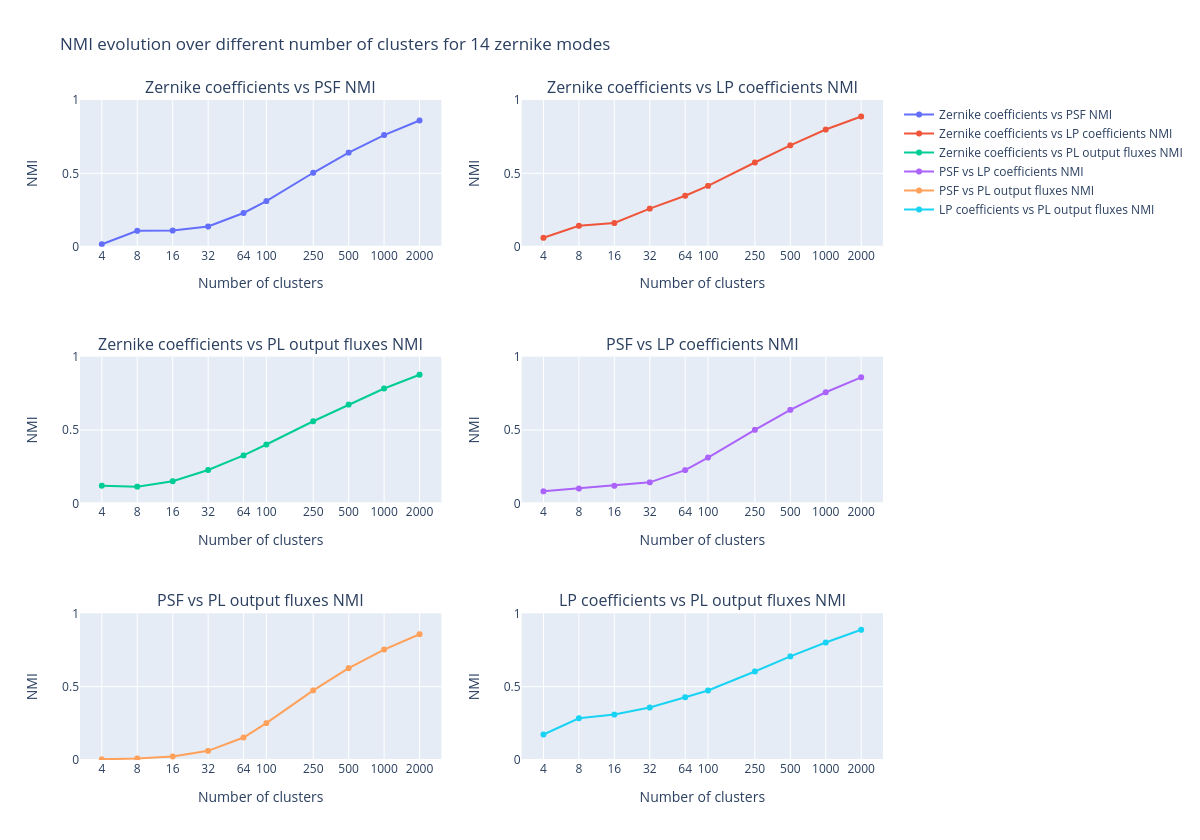
\includegraphics[width=0.9\textwidth]{nmia-nmievolutionover14.png}
		\end{figure*}
		
\begin{table}[h!]
\centering
\begin{tabular}{|c|c|c|c|c|c|c|}
\hline
\textbf{Clusters} & \textbf{Z vs PSF} & \textbf{Z vs LP} & \textbf{Z vs PL} & \textbf{PSF vs LP} & \textbf{PSF vs PL} & \textbf{LP vs PL} \\
\hline
4 & 0.0159 & 0.0597 & 0.1197 & 0.0812 & 0.0037 & 0.1733 \\
8 & 0.1060 & 0.1401 & 0.1117 & 0.0988 & 0.0080 & 0.2831 \\
16 & 0.1026 & 0.1541 & 0.1437 & 0.1123 & 0.0160 & 0.3038 \\
32 & 0.1113 & 0.2371 & 0.2041 & 0.1171 & 0.0340 & 0.3384 \\
64 & 0.1335 & 0.2655 & 0.2428 & 0.1300 & 0.0481 & 0.3567 \\
100 & 0.1239 & 0.2544 & 0.2377 & 0.1264 & 0.0497 & 0.3309 \\
250 & 0.0840 & 0.2105 & 0.1847 & 0.0806 & 0.0323 & 0.2672 \\
500 & 0.0535 & 0.1821 & 0.1361 & 0.0464 & 0.0184 & 0.2267 \\
1000 & 0.0380 & 0.1885 & 0.1261 & 0.0279 & 0.0112 & 0.2024 \\
2000 & 0.0239 & 0.2135 & 0.1380 & 0.0190 & 0.0055 & 0.2160 \\
\hline
\end{tabular}
\caption{AMI Analysis for Different Numbers of Clusters}
\end{table}
		\FloatBarrier
		
	\subsubsection{AMI evolution over number of clusters for 20 zernike mode related datasets}
		\begin{figure*}[ht!]
			\centering
			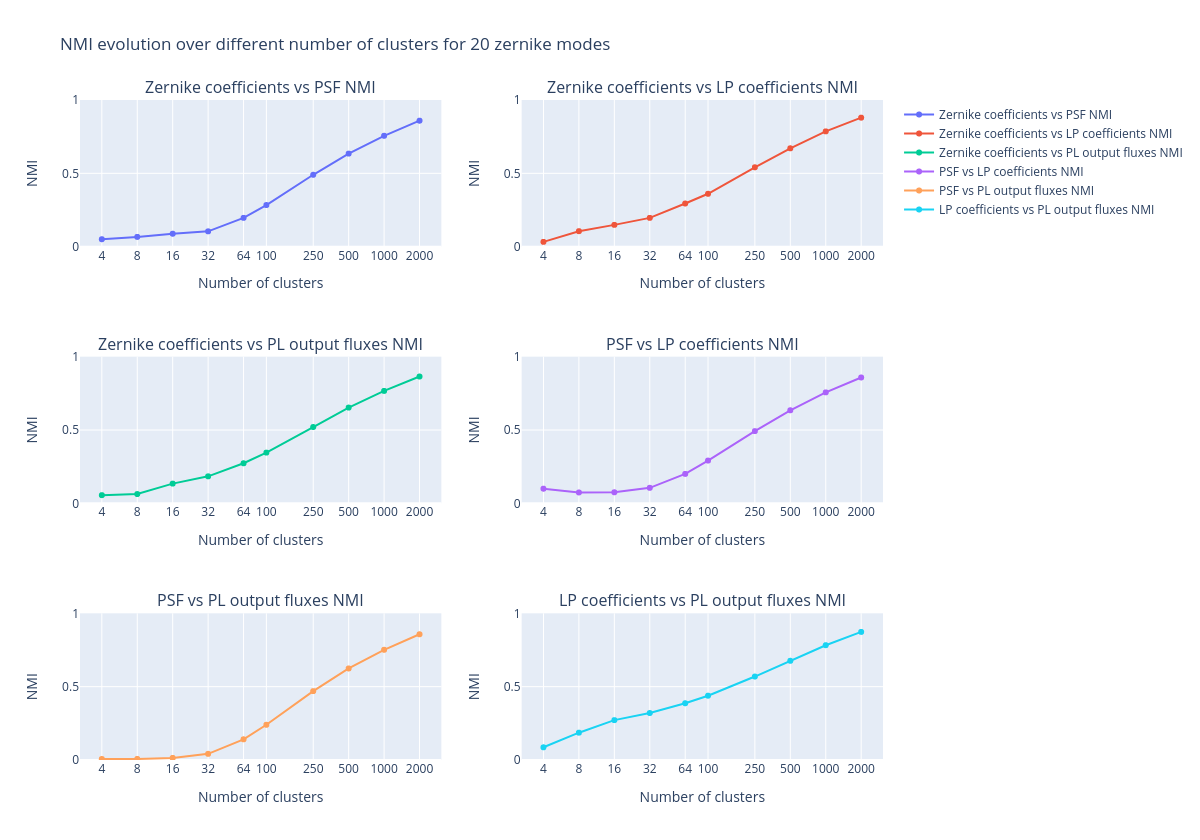
\includegraphics[width=0.9\textwidth]{nmia-nmievolutionover20.png}
		\end{figure*}
		
\begin{table}[h!]
\centering
\begin{tabular}{|c|c|c|c|c|c|c|}
\textbf{Clusters} & \textbf{Z vs PSF} & \textbf{Z vs LP} & \textbf{Z vs PL} & \textbf{PSF vs LP} & \textbf{PSF vs PL} & \textbf{LP vs PL} \\
\hline
4  & 0.0501 & 0.0321 & 0.0549 & 0.0992 & 0.0061 & 0.0861 \\
8  & 0.0644 & 0.1034 & 0.0611 & 0.0719 & 0.0048 & 0.1843 \\ 
16 & 0.0807 & 0.1416 & 0.1273 & 0.0676 & 0.0062 & 0.2657 \\ 
32 & 0.0775 & 0.1721 & 0.1596 & 0.0788 & 0.0131 & 0.2998 \\ 
64 & 0.0960 & 0.2058 & 0.1823 & 0.1008 & 0.0339 & 0.3103 \\ 
100 & 0.0896 & 0.1859 & 0.1676 & 0.0997 & 0.0348 & 0.2855 \\ 
250 & 0.0575 & 0.1513 & 0.1117 & 0.0629 & 0.0200 & 0.2030 \\ 
500 & 0.0391 & 0.1348 & 0.0871 & 0.0397 & 0.0111 & 0.1492 \\ 
1000 & 0.0231 & 0.1485 & 0.0716 & 0.0254 & 0.0071 & 0.1360 \\ 
2000 & 0.0139 & 0.1754 & 0.0685 & 0.0156 & 0.0027 & 0.1343 \\ 
\hline
\end{tabular}
\caption{AMI Analysis for Different Numbers of Clusters}
\end{table}
		\FloatBarrier
		
		
	\subsubsection{AMI evolution over number of clusters for 27 zernike mode related datasets}
		\begin{figure*}[ht!]
			\centering
			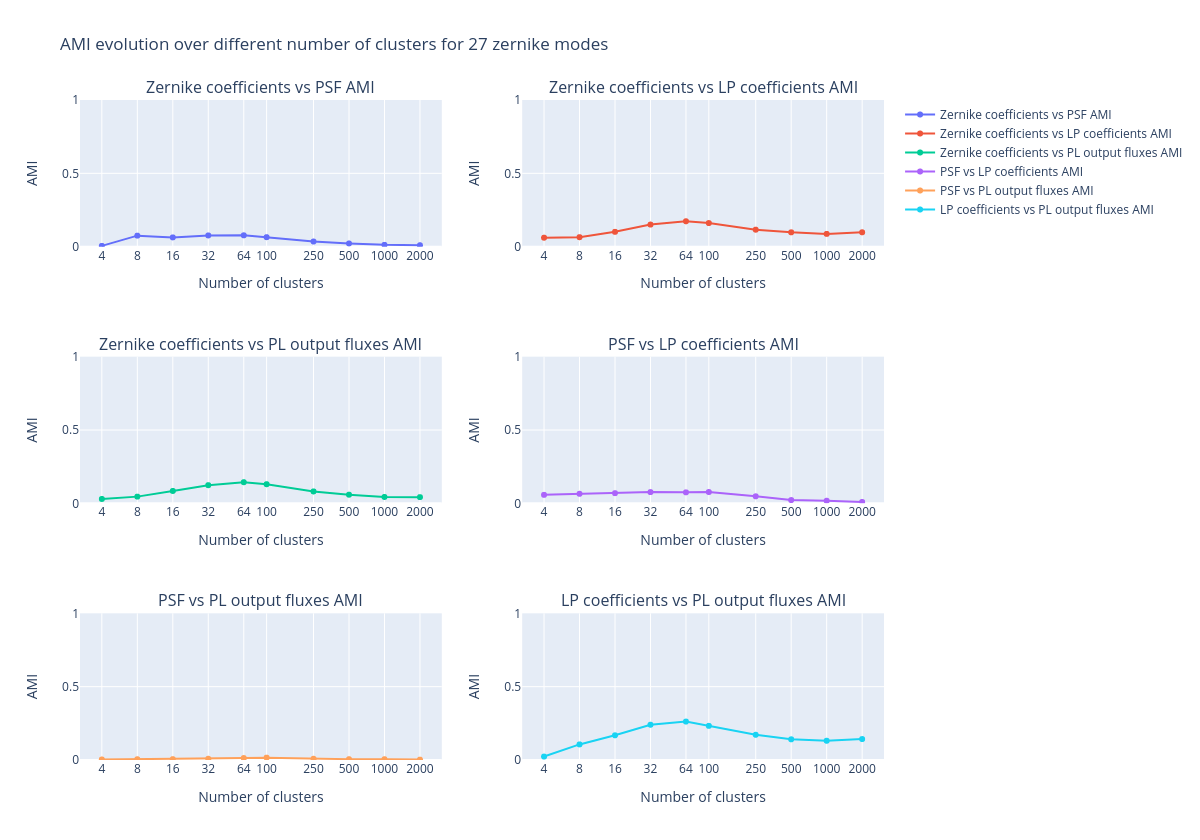
\includegraphics[width=0.9\textwidth]{nmia-nmievolutionover27.png}
		\end{figure*}
		
\begin{table}[h!]
\centering
\begin{tabular}{|c|c|c|c|c|c|c|}
\hline
\textbf{Clusters} & \textbf{Z vs PSF} & \textbf{Z vs LP} & \textbf{Z vs PL} & \textbf{PSF vs LP} & \textbf{PSF vs PL} & \textbf{LP vs PL} \\
\hline
4   & 0.0053 & 0.0610 & 0.0298 & 0.0579 & 0.0034 & 0.0234 \\
8   & 0.0751 & 0.0646 & 0.0458 & 0.0651 & 0.0051 & 0.1063 \\
16  & 0.0631 & 0.1010 & 0.0843 & 0.0693 & 0.0055 & 0.1685 \\
32  & 0.0765 & 0.1506 & 0.1237 & 0.0767 & 0.0083 & 0.2404 \\
64  & 0.0773 & 0.1732 & 0.1440 & 0.0748 & 0.0132 & 0.2621 \\
100 & 0.0646 & 0.1610 & 0.1303 & 0.0771 & 0.0161 & 0.2329 \\
250 & 0.0352 & 0.1157 & 0.0811 & 0.0480 & 0.0084 & 0.1721 \\
500 & 0.0218 & 0.0978 & 0.0589 & 0.0223 & 0.0054 & 0.1410 \\
1000& 0.0123 & 0.0871 & 0.0434 & 0.0177 & 0.0053 & 0.1313 \\
2000& 0.0097 & 0.0979 & 0.0423 & 0.0092 & 0.0026 & 0.1428 \\
\hline
\end{tabular}
\caption{AMI Analysis for Different Numbers of Clusters}
\end{table}
		\FloatBarrier
		
	
	\subsubsection{AMI evolution over number of clusters for 35 zernike mode related datasets}
		\begin{figure*}[ht!]
			\centering
			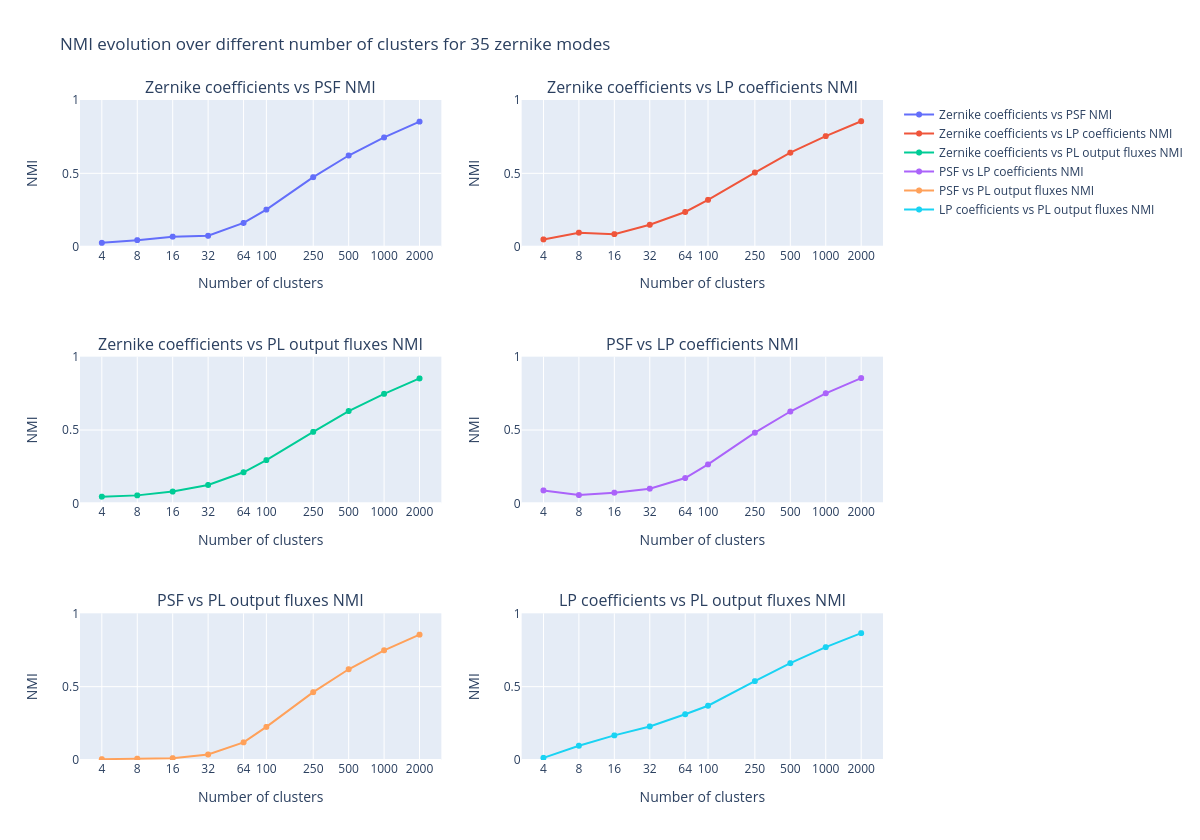
\includegraphics[width=0.9\textwidth]{nmia-nmievolutionover35.png}
		\end{figure*}
		
\begin{table}[h!]
\centering
\begin{tabular}{|c|c|c|c|c|c|c|}
\hline
\textbf{Clusters} & \textbf{Z vs PSF} & \textbf{Z vs LP} & \textbf{Z vs PL} & \textbf{PSF vs LP} & \textbf{PSF vs PL} & \textbf{LP vs PL} \\
\hline
4    & 0.0255 & 0.0489 & 0.0449 & 0.0875 & 0.0050 & 0.0142 \\ 
8    & 0.0422 & 0.0933 & 0.0520 & 0.0542 & 0.0068 & 0.0952 \\ 
16   & 0.0606 & 0.0779 & 0.0727 & 0.0650 & 0.0045 & 0.1609 \\ 
32   & 0.0463 & 0.1237 & 0.0989 & 0.0728 & 0.0083 & 0.2056 \\ 
64   & 0.0571 & 0.1409 & 0.1131 & 0.0690 & 0.0104 & 0.2260 \\ 
100  & 0.0509 & 0.1333 & 0.1026 & 0.0669 & 0.0169 & 0.1983 \\ 
250  & 0.0308 & 0.0858 & 0.0527 & 0.0438 & 0.0091 & 0.1446 \\ 
500  & 0.0188 & 0.0671 & 0.0392 & 0.0227 & 0.0054 & 0.1121 \\ 
1000 & 0.0085 & 0.0595 & 0.0282 & 0.0166 & 0.0031 & 0.1025 \\ 
2000 & 0.0066 & 0.0572 & 0.0247 & 0.0056 & 0.0026 & 0.1428 \\ 
\hline
\end{tabular}
\caption{AMI Analysis for Different Numbers of Clusters}
\end{table}
		\FloatBarrier
		
		
	\subsubsection{AMI evolution over number of clusters for 44 zernike mode related datasets}
		\begin{figure*}[ht!]
			\centering
			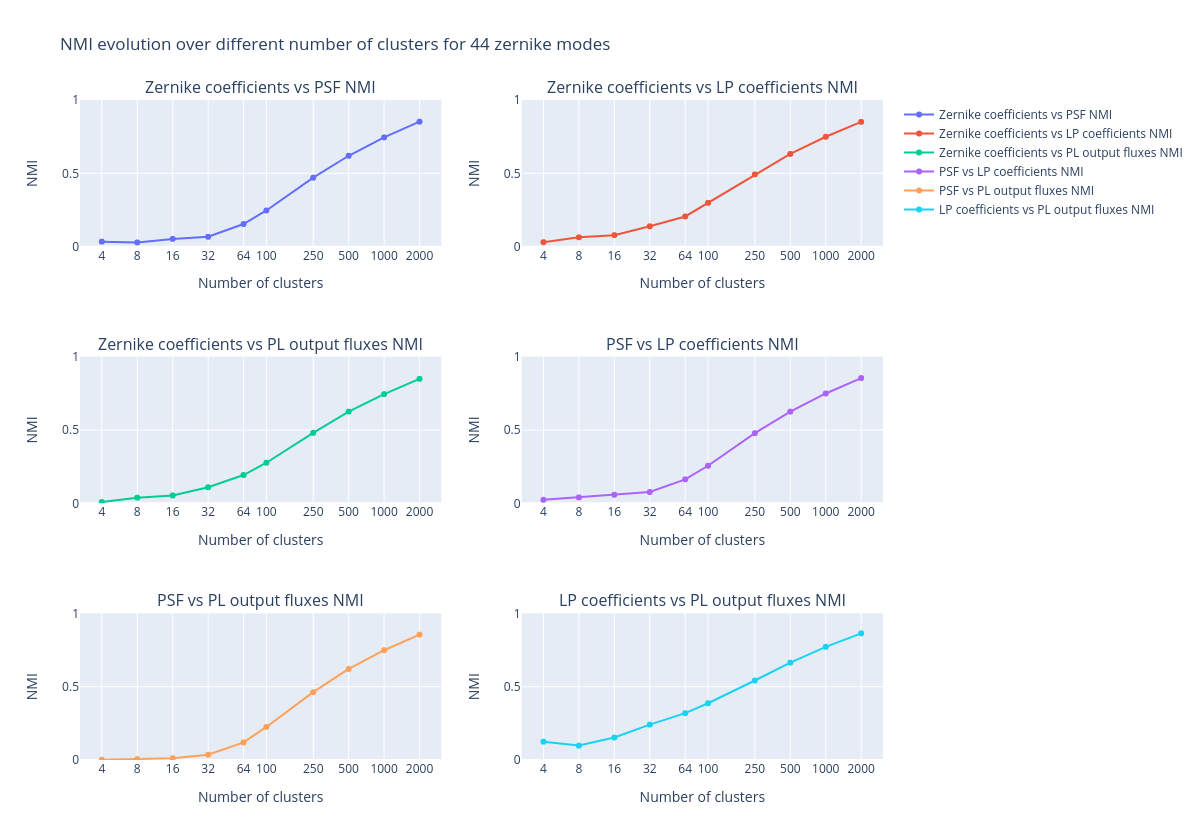
\includegraphics[width=0.9\textwidth]{nmia-nmievolutionover44.png}
		\end{figure*}
		
\begin{table}[h!]
\centering
\begin{tabular}{|c|c|c|c|c|c|c|}
\hline
\textbf{Clusters} & \textbf{Z vs PSF} & \textbf{Z vs LP} & \textbf{Z vs PL} & \textbf{PSF vs LP} & \textbf{PSF vs PL} & \textbf{LP vs PL} \\
\hline
4   & 0.0336 & 0.0299 & 0.0081 & 0.0235 & 0.0012 & 0.1244 \\ 
8   & 0.0266 & 0.0613 & 0.0363 & 0.0381 & 0.0037 & 0.0961 \\ 
16  & 0.0453 & 0.0709 & 0.0458 & 0.0506 & 0.0038 & 0.1460 \\ 
32  & 0.0391 & 0.1129 & 0.0829 & 0.0493 & 0.0067 & 0.2184 \\ 
64  & 0.0491 & 0.1066 & 0.0920 & 0.0593 & 0.0101 & 0.2344 \\ 
100 & 0.0428 & 0.1070 & 0.0796 & 0.0546 & 0.0159 & 0.2195 \\ 
250 & 0.0262 & 0.0648 & 0.0447 & 0.0363 & 0.0091 & 0.1528 \\
500 & 0.0124 & 0.0481 & 0.0293 & 0.0197 & 0.0066 & 0.1227 \\ 
1000 & 0.0093 & 0.0438 & 0.0207 & 0.0112 & 0.0031 & 0.1112 \\ 
2000 & 0.0045 & 0.0368 & 0.0159 & 0.0079 & 0.0019 & 0.1019 \\ 
\hline
\end{tabular}
\caption{AMI Analysis for Different Numbers of Clusters}
\end{table}
		\FloatBarrier
		
		
	\subsubsection{AMI evolution over number of zernike modes}
	
	\begin{figure*}[ht!]
			\centering
			\subfloat[AMI evolution over number of clusters for Zernike coefficients vs PSF]{%
				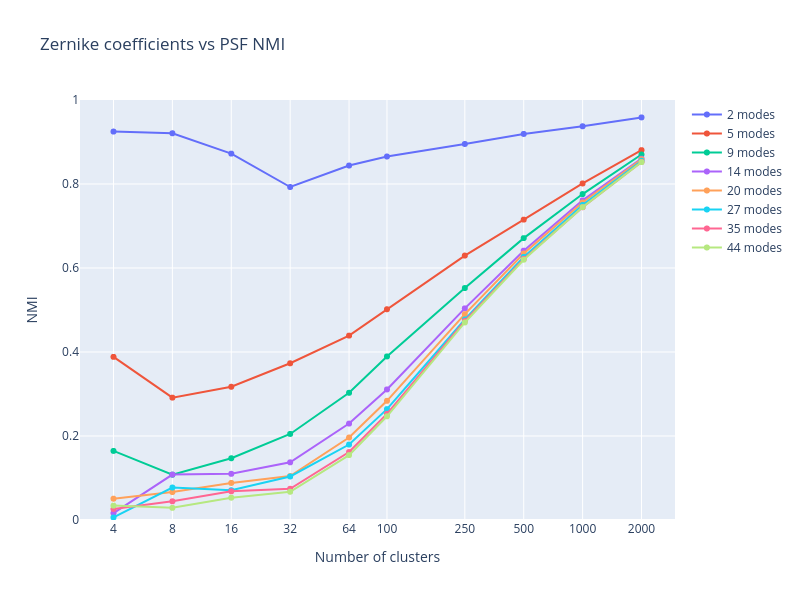
\includegraphics[width=0.45\textwidth]{nmia-zernikecoefficientsvspsfnmi.png}}
			\hspace{\fill}
			\subfloat[AMI evolution over number of clusters for Zernike coefficients vs LP coefficients]{%
				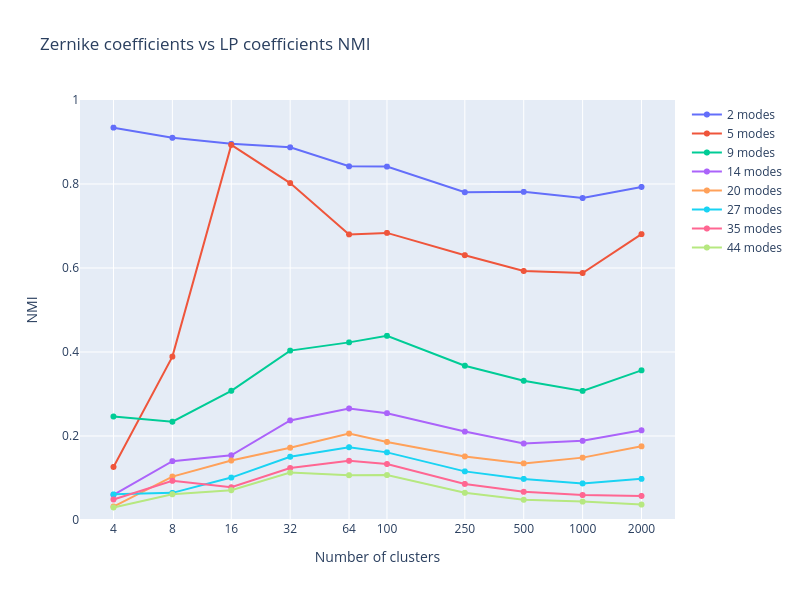
\includegraphics[width=0.45\textwidth]{nmia-zernikecoefficientsvslpcoefficientsnmi.png}}
			\\
			\subfloat[AMI evolution over number of clusters for Zernike coefficients vs PL output fluxes]{%
				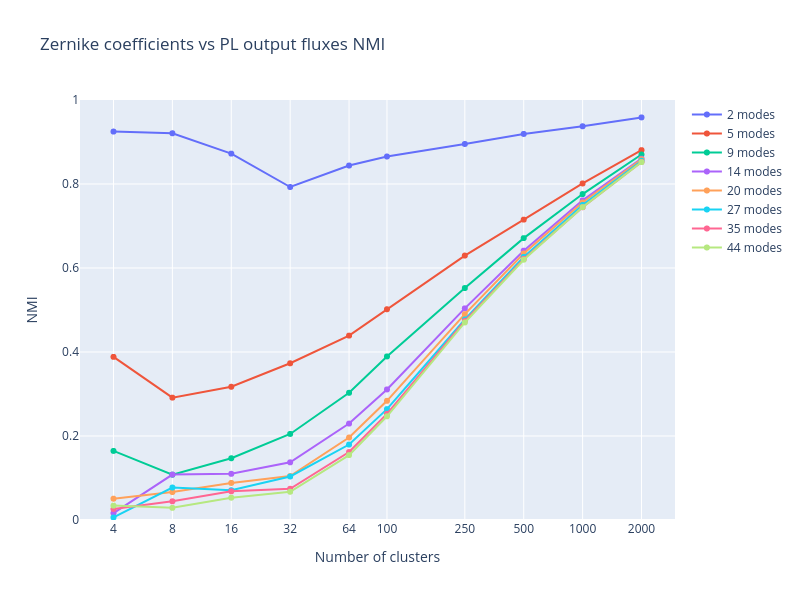
\includegraphics[width=0.45\textwidth]{nmia-zernikecoefficientsvsploutputfluxesnmi.png}}
			\hspace{\fill}
			\subfloat[AMI evolution over number of clusters for PSF vs LP coefficients]{%
				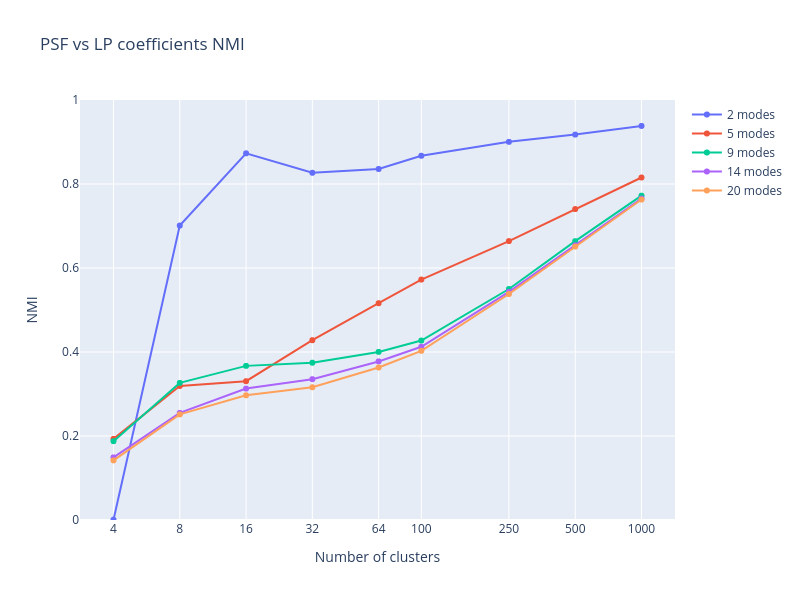
\includegraphics[width=0.45\textwidth]{nmia-psfvslpcoefficientsnmi.png}}
			\\
			\subfloat[AMI evolution over number of clusters for PSF vs PL output fluxes]{%
				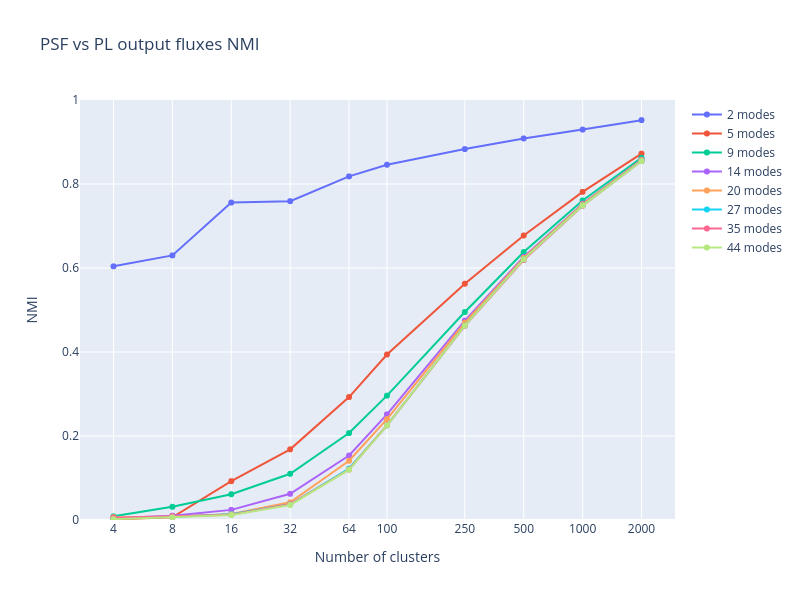
\includegraphics[width=0.45\textwidth]{nmia-psfvsploutputfluxesnmi.png}}
			\hspace{\fill}
			\subfloat[AMI evolution over number of clusters for LP coefficients vs PL output fluxes]{%
				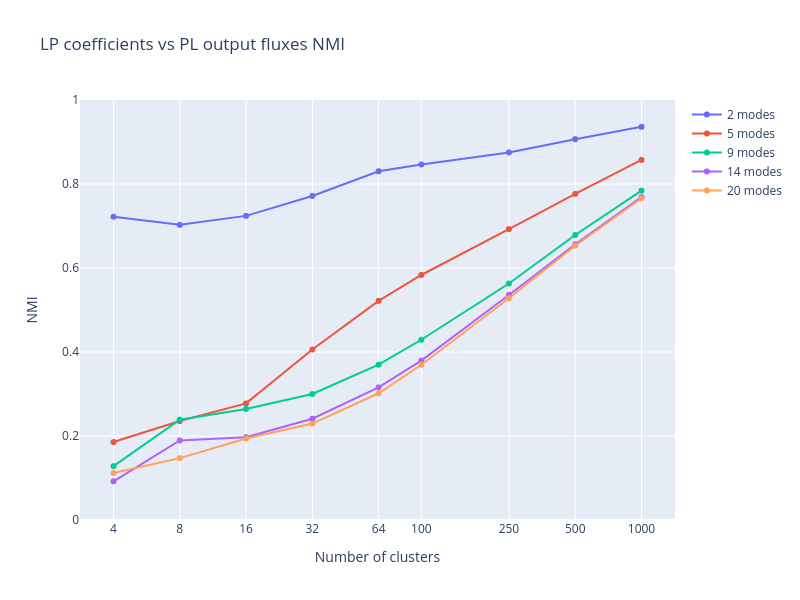
\includegraphics[width=0.45\textwidth]{nmia-lpcoefficientsvsploutputfluxesnmi.png}}
		\end{figure*}
		

		\FloatBarrier